\chapter{Comparison of MOR Methods} \label{analysis}
The previously mentioned methods for model order reduction will be compared regarding time domain error, frequency domain error and computational speed.
The time domain error will be obtained by comparing the FEM solution to a given approximation.
To get insights into the frequency domain error, the error system of a reduced order model will be analysed.
The computational speed will be determined by measuring the time it takes to generate a ROM.
Here it is assumed that the implementations provided by MORLAB are programmed in a sufficiently effective manner.
For testing the following parameters are used
\begin{gather}
\alpha = 0.1, \quad T = 1, \quad L = 1 \\
n = 100, \quad n_t = 10^{4}
\end{gather}
.

These values are chosen such that it yields results in a timely manner.
Especially \(n_t\) and \(\alpha\) are important for stability of euler scheme.
If both are too low, the euler scheme becomes unstable.
Choosing \(n_t\) too high the time and memory consumption becomes rather large.
There was no exact method for determining the parameters in this way.

\section{Time Domain Error}
The time domain error will defined as \(\epsilon = Y - \hat{Y}\) where \(Y\) and \(\hat{Y}\) denote the matrices storing the output of the systems \(G\) and \(G_r\).
Since the output matrices are usually rather large, it is impractical to use \(\epsilon\) directly.
Therefore  \(||\epsilon||_{F}\) will be considered.
The error is measured using the Frobenius norm to get a measure of the error that respects all data points.
Here two aspects are interesting.
There will be two different initial conditions considered.
The first one is \(x(0, x) = 1\).
It is chosen in this way to display the workings of the boundary condition.
If there were no boundary conditions, for a constant initial condition the system would never cool down since \(\frac{\partial^2 u}{\partial x^2} = 0\) (\ref{eq-1d-h}) at every point in time.
This only holds if there is no input to the system.
Therefore \(u(t) = 0\), where \(u\) denotes the systems input.
The second initial condition is \(x(0, x) = \sin(\frac{2\pi}{L}x)\) with random input.
The initial condition is sinusoidal since it is easy to approximate.
\pagebreak
\subsection{Proper Orthogonal decomposition}
Figure \ref{FIG-ERR-POD} shows the \(L2\) error of the solution obtained by the POD model.
\begin{figure}[H]
\centering
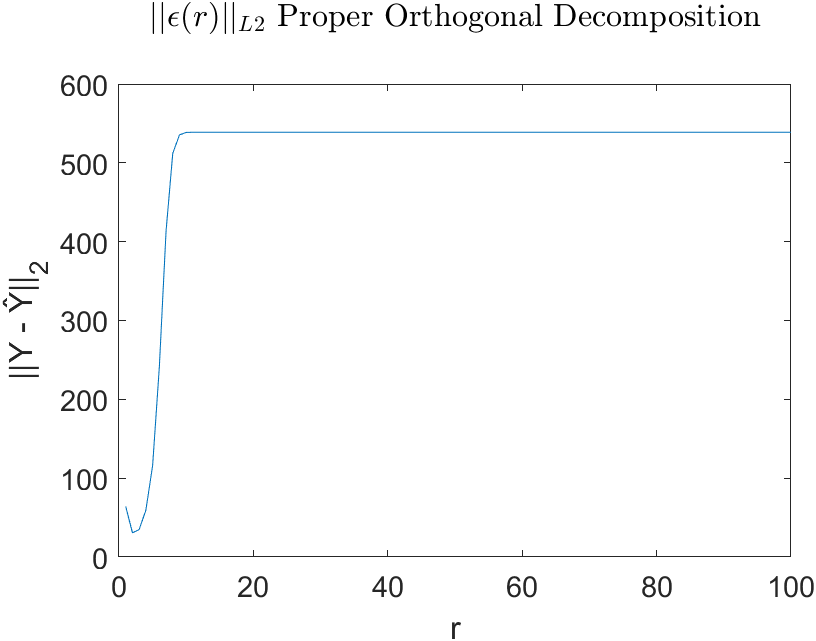
\includegraphics[width=12.5cm]{images/L2_POD}
\caption{L2 Error Proper Orthogonal Decomposition $x(0, x) = 1$}
\label{FIG-ERR-POD}
\end{figure}
It is clearly visible that the error is minimal at  \(r=2\).
This is to be expected since for large \(r\) also low variance modes will be included.
Figure \ref{FIG-POD-VAR} shows that the first two modes capture the most variance with roughly 96\% combined.
It is also visible that all the remaining modes combined only capture 4\%.
\begin{figure}[H]
\centering
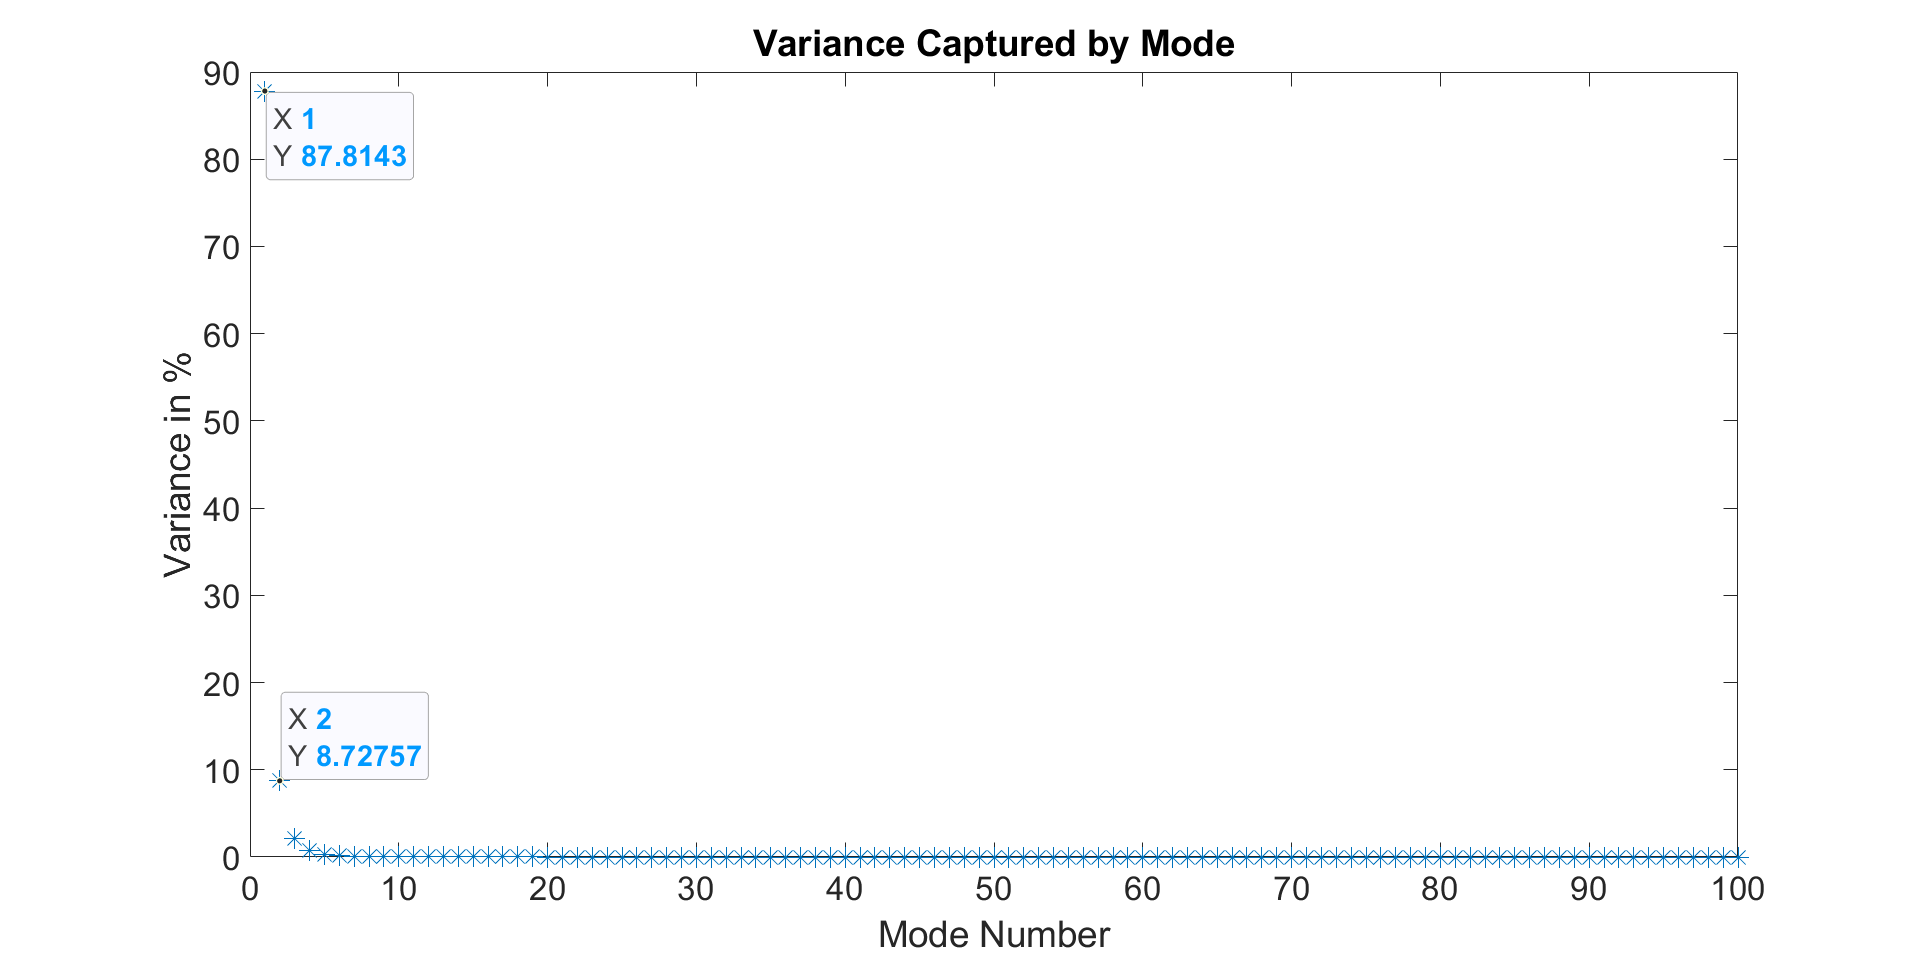
\includegraphics[width=12.5cm]{images/test_modes_pod}
\caption{Variance of POD Modes}
\label{FIG-POD-VAR}
\end{figure}
In this case the low variance modes introduce error, since the initial condition is poorly approximated using orthogonal basis vectors.
This can be seen on figure \ref{fig-pod-100}.
\begin{figure}[H]
\begin{subfigure}[b]{0.5\textwidth}
\centering
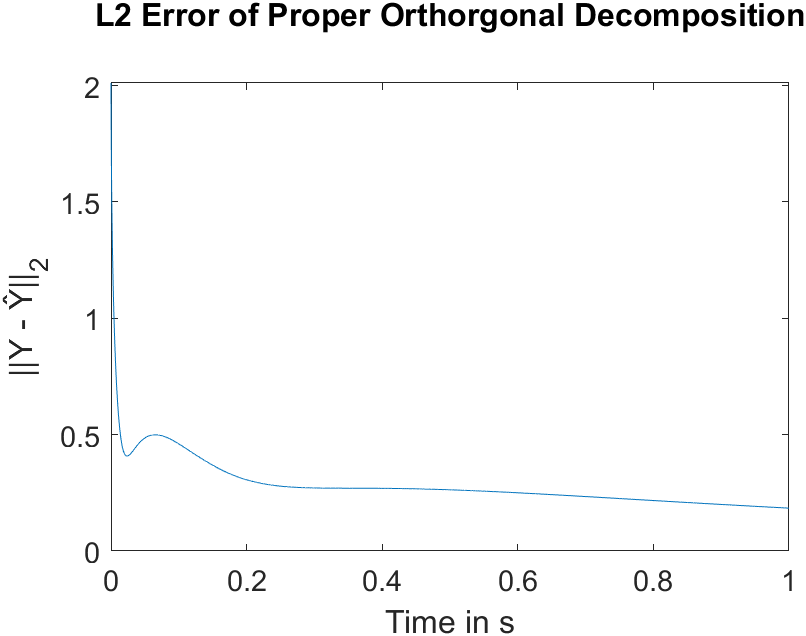
\includegraphics[width=\textwidth]{images/L2_Proper Orthorgonal Decomposition_2_100}
\caption{L2 POD error $r=2$, $n=100$, $x(0, x) = 1$}
\label{fig:fig-pod-2-100}
\end{subfigure}
\begin{subfigure}[b]{0.5\textwidth}
\centering
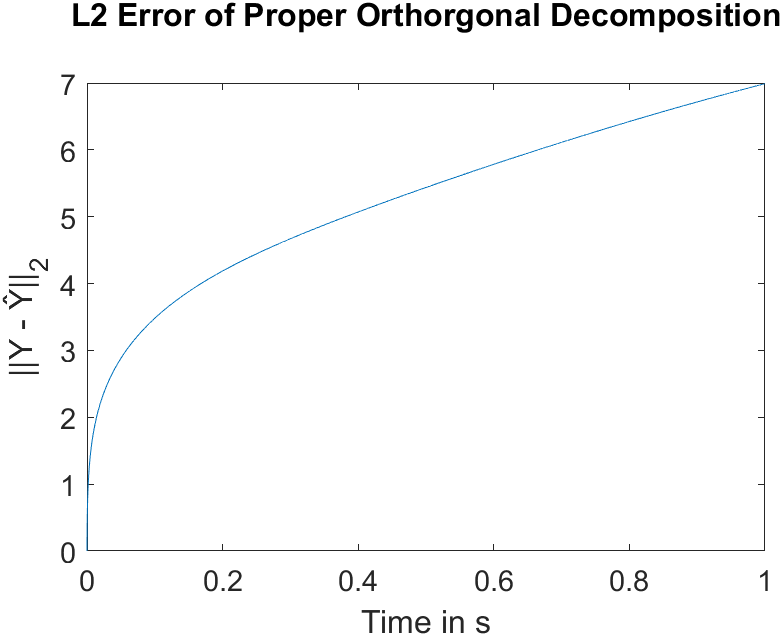
\includegraphics[width=\textwidth]{images/L2_Proper Orthorgonal Decomposition_100_100}
\caption{L2 POD error $r=100$, $n=100$, $x(0, x) = 1$}
\label{fig:fig-pod-100-100}
\end{subfigure}
\label{fig-pod-100}
\end{figure}
The \(L2\) error for \(r=2\) can be seen on \ref{fig:fig-pod-2-100}.
Here for \(t=0\) the error is the largest and then drops of quickly and seems to converge to roughly 0.3 whereas the error on \ref{fig:fig-pod-100-100} for \(r=100\) is almost zero at \(t=0\) and diverges.
This problem does not only apply to the initial condition, this problem if the snapshot matrix contains vectors that are poorly approximated using orthogonal basis vectors.
The low variance modes do not introduce error. 
In fact they even lower the error and the error is lower in general as it can be seen on figure \ref{FIG-ERR-POD-SIN}.
\begin{figure}[H]
\centering
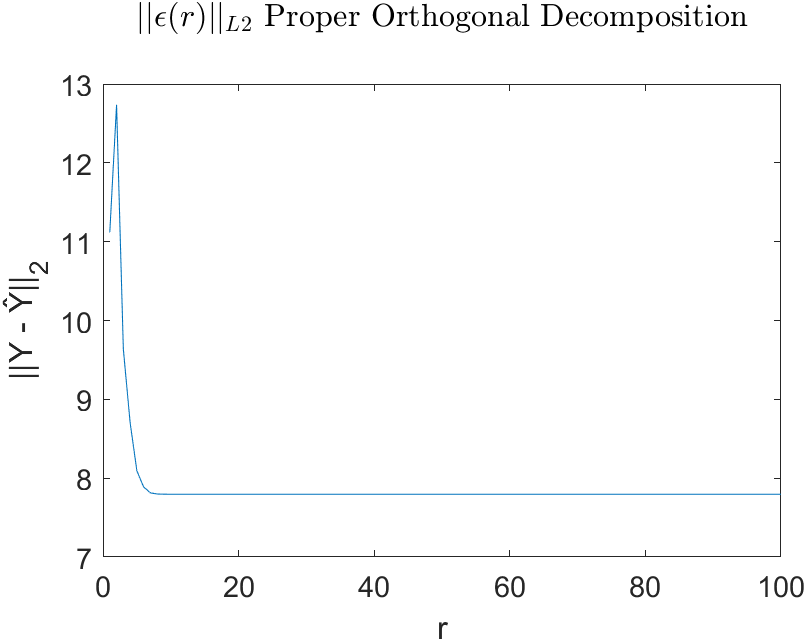
\includegraphics[width=12.5cm]{images/L2_POD_SIN}
\caption{L2 Error Proper Orthogonal Decomposition $x(0, x) = \sin(\frac{2\pi}{L}x)$}
\label{FIG-ERR-POD-SIN}
\end{figure}
Another difference is that for $x(0, x) = \sin(\frac{2\pi}{L}x)$ the error distribution over time does not differ as much for \(r=100\) and \(r=2\).
This can be observed on figure \ref{fig:fig-pod-2-100-sina} and \ref{fig:fig-pod-100-100-sinb}.
\begin{figure}[H]
\begin{subfigure}[b]{0.5\textwidth}
\centering
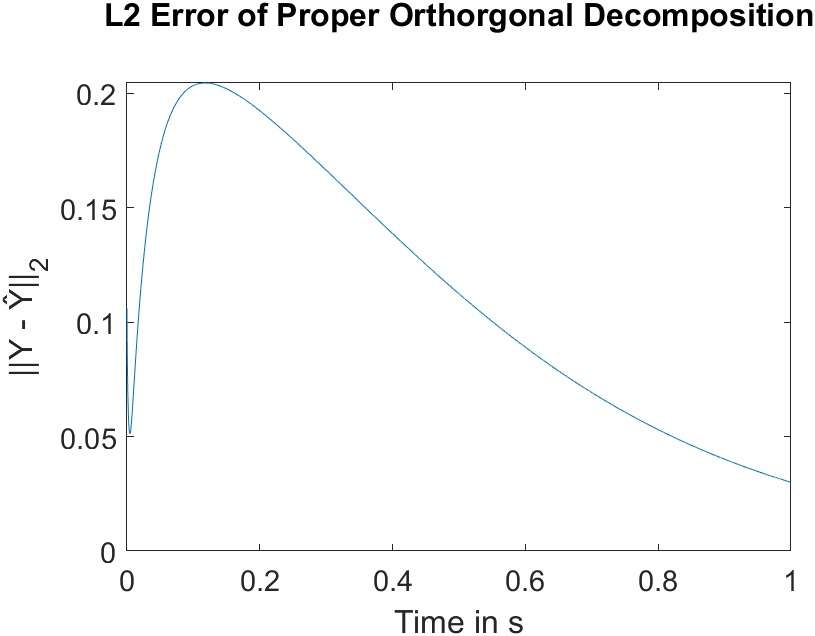
\includegraphics[width=\textwidth]{images/L2_Proper Orthorgonal Decomposition_2_100sin}
\caption{ $r=2$, $n=100$, $x(0, x) = \sin(\frac{2\pi}{L}x)$}
\label{fig:fig-pod-2-100-sina}
\end{subfigure}
\begin{subfigure}[b]{0.5\textwidth}
\centering
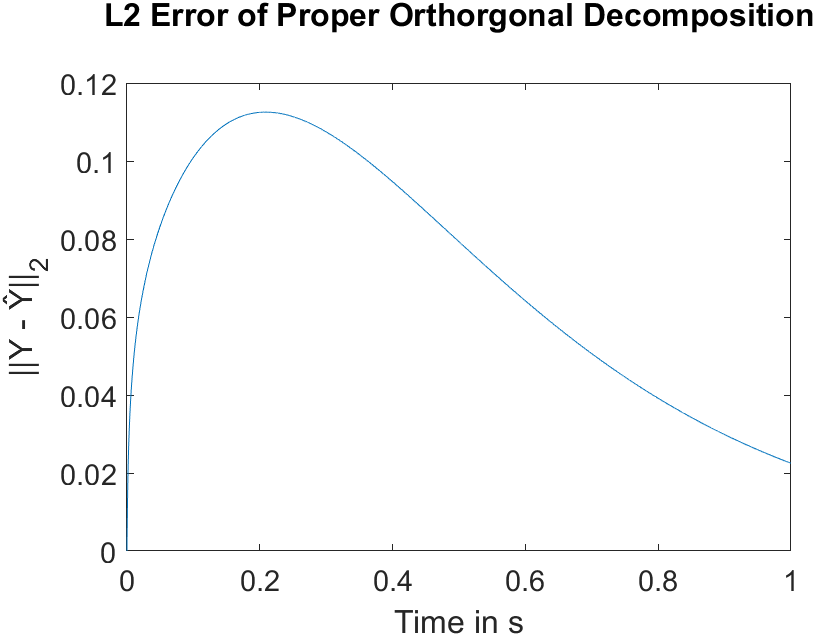
\includegraphics[width=\textwidth]{images/L2_Proper Orthorgonal Decomposition_100_100sin}
\caption{$r=100$, $n=100$, $x(0, x) = \sin(\frac{2\pi}{L}x)$}
\label{fig:fig-pod-100-100-sinb}
\end{subfigure}
\label{fig-pod-100-sin}
\caption{L2 POD error}
\end{figure}


\subsection{Modal Truncation}
Figure \ref{FIG-ERR-MT} shows the \(L2\) error of the ROM obtained by Modal Truncation.
\begin{figure}[H]
\begin{subfigure}[b]{0.5\textwidth}
\centering
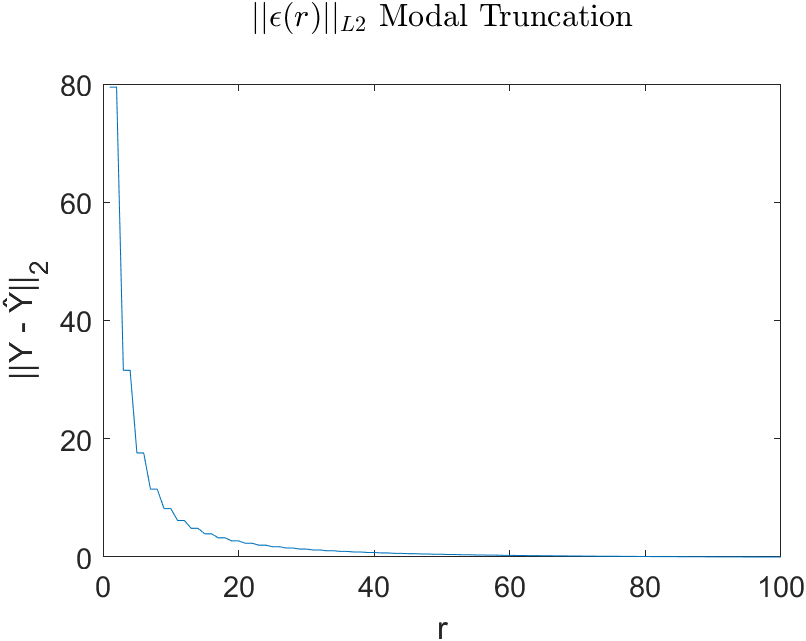
\includegraphics[width=\textwidth]{images/L2_MT}
\caption{$x(0, x) = 1$}
\label{FIG-ERR-MT}
\end{subfigure}
\begin{subfigure}[b]{0.5\textwidth}
\centering
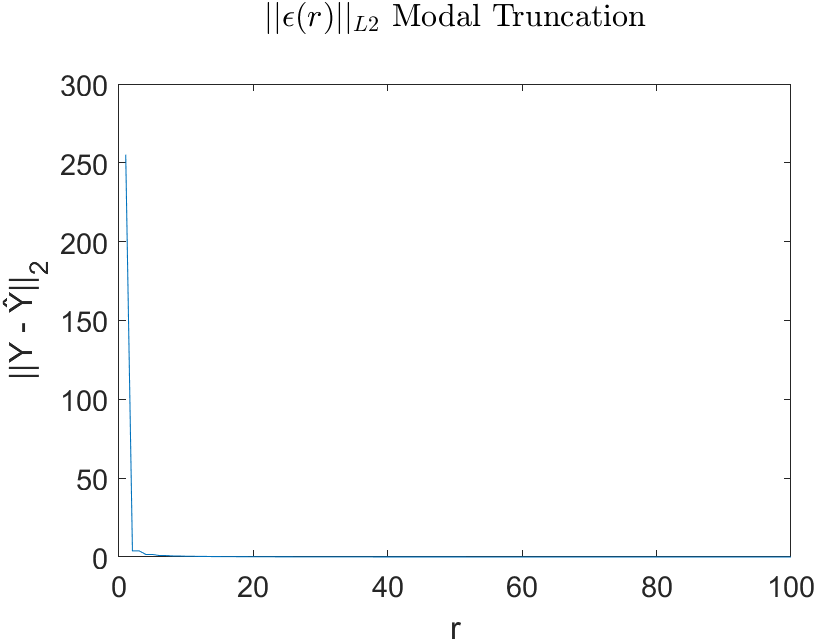
\includegraphics[width=\textwidth]{images/L2_MT_SIN}
\caption{$x(0, x) = \sin(\frac{2\pi}{L}x)$}
\label{FIG-ERR-MT-SIN}
\end{subfigure}
\caption{L2 Error Balanced Truncation}
\end{figure}
It shows that as \(r\) increases the error converges to zero.
This is to be expected since as \(r\) increases \(G_r\) becomes closer to \(G\).
For \(x(0, x) = \sin(\frac{2\pi}{L}x)\) the error starts off significantly higher but decays even faster as it can be seen on figure \ref{FIG-ERR-MT-SIN}.

\subsection{Balanced Truncation}
Figure \ref{FIG-ERR-BT} shows the \(L2\) error of the ROM obtained by Balanced Truncation.


\begin{figure}[H]
\begin{subfigure}[b]{0.5\textwidth}
\centering
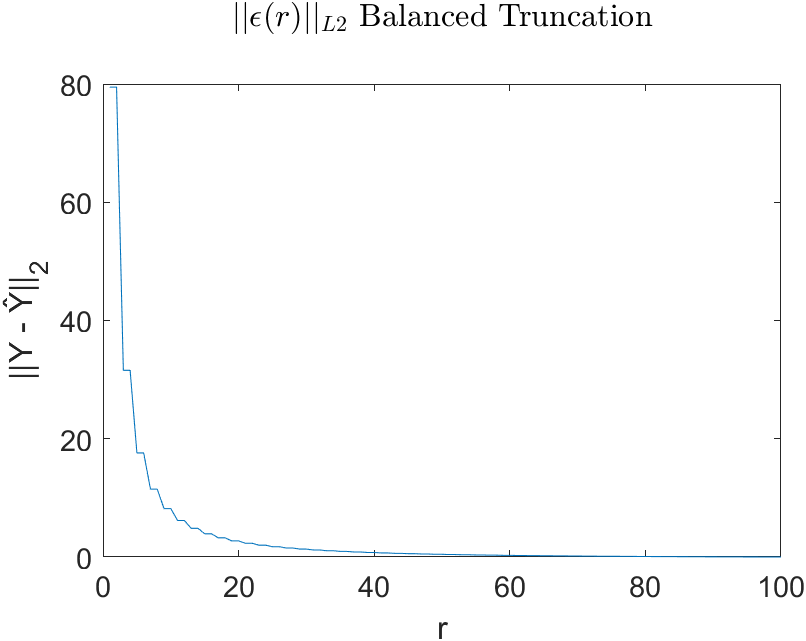
\includegraphics[width=\textwidth]{images/L2_BT}
\caption{$x(0, x) = 1$}
\label{FIG-ERR-BT}
\end{subfigure}
\begin{subfigure}[b]{0.5\textwidth}
\centering
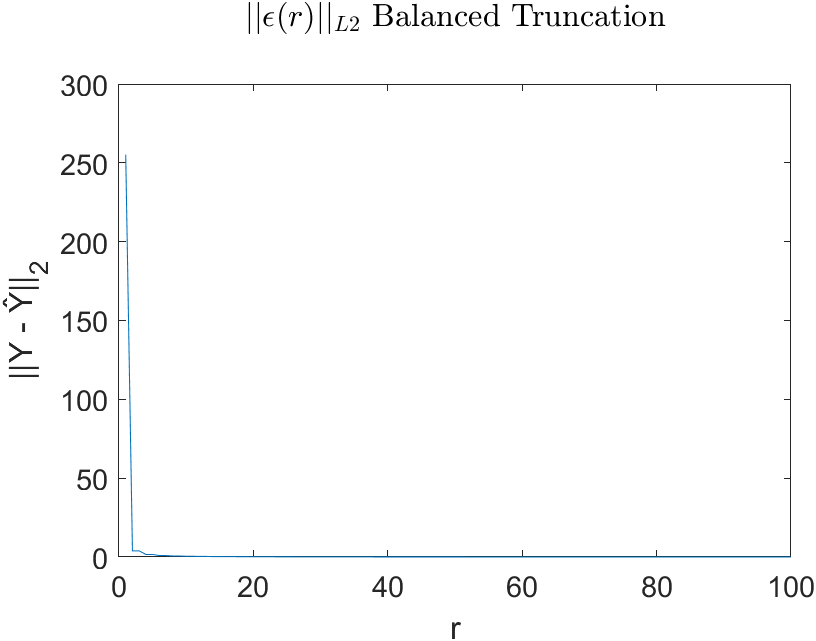
\includegraphics[width=\textwidth]{images/L2_BT_SIN}
\caption{$x(0, x) = \sin(\frac{2\pi}{L}x)$}
\label{FIG-ERR-BT-SIN}
\end{subfigure}
\caption{L2 Error Balanced Truncation}
\end{figure}
It shows that as \(r\) increases the error converges to zero.
This is to be expected since as \(r\) increases \(G_r\) becomes closer to \(G\).

It is remarkable that \ref{FIG-ERR-BT} is identical to \ref{FIG-ERR-MT}.
At the end of this chapter

\subsection{Hankel Norm Approximation}
Figure \ref{FIG-ERR-HNA} shows the \(l2\) error of the output generated by the HNA model.
Here it is striking that for \(r > \frac{n}{3}\) the model does not generate usable output.
However for \(r \leq \frac{n}{3}\) the error converges to zero as \(r\) increases.

\begin{figure}[H]
\begin{subfigure}[b]{0.5\textwidth}
\centering
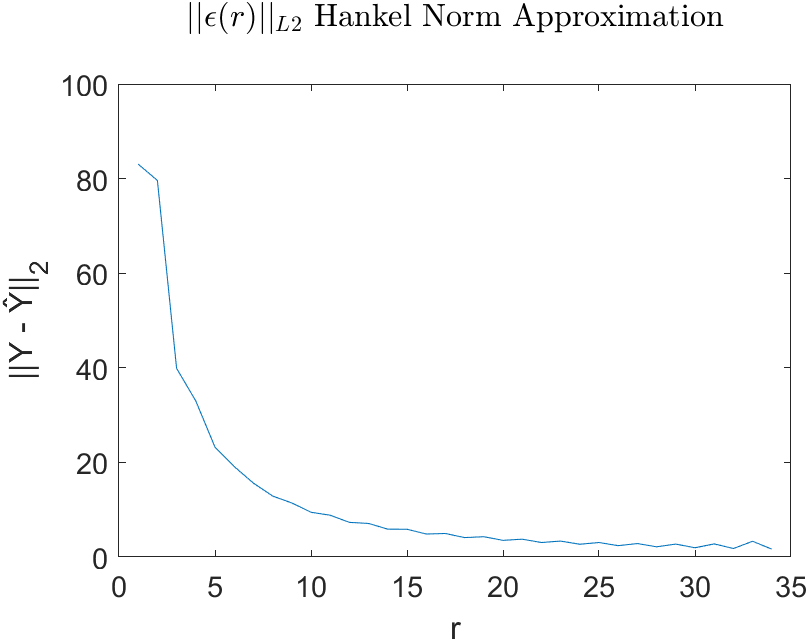
\includegraphics[width=\textwidth]{images/L2_HNA}
\caption{$x(0, x) = 1$}
\label{FIG-ERR-HNA}
\end{subfigure}
\begin{subfigure}[b]{0.5\textwidth}
\centering
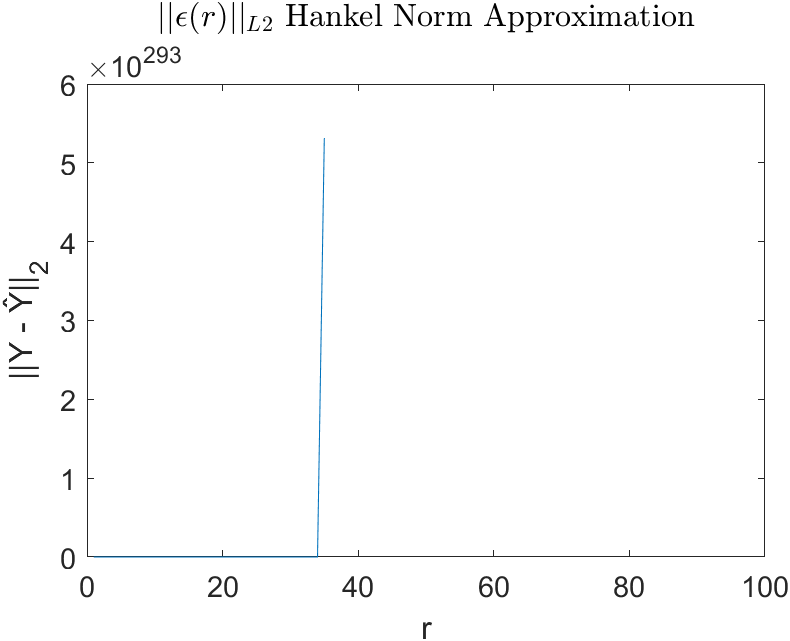
\includegraphics[width=\textwidth]{images/L2_HNA_SIN}
\caption{$x(0, x) = \sin(\frac{2\pi}{L}x)$}
\label{FIG-ERR-HNA-SIN}
\end{subfigure}
\caption{L2 Error Balanced Truncation}
\end{figure}
It is noticeable that similar to BT and MT the error for \(x(0, x) = \sin(\frac{2\pi}{L}x)\) starts higher than for \(x(0, x) = 1\) and then decays quite fast.

\subsection{Modal Truncation is Equal to Balanced Truncation}
The results for BT and MT are the same since \(B = C\) and \(A\) is symmetric.
Remember that \(A^{n\times n} = M^{-1}K\) where both \(K\) and \(M\) are symmetric, hence \(A\) is symmetric \cite{170372}.
The eigenvectors of a symmetric matrix are mutually orthogonal \cite{Zhang}.
Therefore the eigendecomposition of  \(A\) is
\begin{gather}
AX = X\Delta
\end{gather}.
The eigenvalues of a symmetric matrix are real .
It is assumed that \(\Delta = diag(\lambda_1, ..., \lambda_n)\) with \(\lambda_1 \geq \lambda_2 \geq ... \geq \lambda_n\).
where \(XX^T = X^TX = I\).
By applying \(x = X\zeta\) to the system, the system becomes
\begin{gather}
\dot{\zeta} = \Delta \zeta + X^{T}u(t) \label{sys-zeta1}\\
\zeta = X\zeta + Du(t) \label{sys-zeta2}
\end{gather}
The grammians of that systems are
\begin{gather}
W_c = \lim_{t \to \infty} \int_{0}^{t} e^{\Delta\tau}Ie^{\Delta\tau}d\tau \label{gramc} \\
= \lim_{t \to \infty} \int_{0}^{t} e^{2\Delta\tau}d\tau \\
= \lim_{t \to \infty} (e^{\Delta t} - I)\Delta^{-1} \\
W_o = \lim_{t \to \infty} \int_{0}^{t} e^{\Delta\tau}Ie^{\Delta\tau}d\tau \label{gramo} \\
= \lim_{t \to \infty} \int_{0}^{t} e^{2\Delta\tau}d\tau \\
= \lim_{t \to \infty} (e^{\Delta t} - I)\Delta^{-1}
\end{gather}
Therefore \(W_c = W_o\), where \(W_c\) and \(W_o\) are diagonal for stable systems.
Since the transfer of heat is a stable process, it is assumed that the according system is stable.
\begin{gather}
W_c = W_o = \lim_{t \to \infty} (e^{\Delta t} - I)\Delta^{-1} \\
= -\Delta^{-1} 
\end{gather}
\cite{658289}
\begin{gather}
W_C = W_o = \begin{bmatrix}
\frac{-1}{\lambda_1} && 0 && \hdots && 0 \\
0 && \frac{-1}{\lambda_2}&& 0 && \vdots \\
\vdots && 0 && \ddots && \vdots \\
0 && 0 && \hdots && \frac{-1}{\lambda_n}
\end{bmatrix}
\end{gather}
This shows that the eigenvectors of \(A\) satisfy the conditions for balancing transformation \(T\) in section \ref{bt}.
Since the eigenvalues are all negative and real the order \(\delta_{11} \geq \delta_{22} \geq ...  \delta_{nn}\) applies.
This enables the mode truncation described in section \ref{bt}.
\begin{gather}
\tilde{x} = \begin{bmatrix}
\zeta_1 \\
\vdots \\
\zeta_r
\end{bmatrix} \quad 
\tilde{z} = \begin{bmatrix}
\zeta_{r+1} \\
\vdots \\
\zeta_n
\end{bmatrix} \quad
z = \begin{bmatrix}
\tilde{x} \\
\tilde{z}
\end{bmatrix}\\
X= \begin{bmatrix}
X_r && X_{n-r}
\end{bmatrix} \quad
X^{-1} = \begin{bmatrix}
X_r^{*} \\
X_{n-r}
\end{bmatrix} \\
\frac{d\tilde{x}}{dt} = \Delta_r \tilde{x} + X^{-1}_ru \\
y = X_r\tilde{x} + Du 
\end{gather}
The transfer function of that system is
\begin{gather}
G(s) = X_r(sI - \Delta_r^{-1})X_r^{T}+D = X_r diag(\frac{1}{s-\lambda_1}, ..., \frac{1}{s-\lambda_r})X_r^{T}+D \\
= \sum_{i=1}^{r} \frac{1}{s-\lambda_i} + D
\end{gather}
This resembles the DCNF of that system where the terms corresponding to the \(n-r\) smallest eigenvalues are truncated.
As shown in section \ref{mtht} this is the optimal modal truncation.
Therefore modal truncation and balanced truncation yields the same system.






